% ============================================================
% ANEXOS
% ============================================================

\chapter{Especificación de Requerimientos de Software (Versión Mejorada)}
\label{anexo:ers}

\noindent Este anexo corresponde a la versión mejorada del documento de especificación de requerimientos (ERS) del sistema, elaborado con base en la plantilla Volere \cite{ref23} y aprobado en el parcial anterior. Debe ser consistente con el diseño presentado en las Secciones A, B y C de este documento.

\bigskip
\noindent\textbf{Opción 1 -- Adjuntar como PDF independiente ya diagramado:}\\
Si el ERS mejorado ya está en un PDF aparte, descomente la siguiente línea y coloque el archivo en \texttt{imagenes/ers\_mejorado.pdf}:
%\includepdf[pages=-,pagecommand={}]{imagenes/ers_mejorado.pdf}

\bigskip
\noindent\textbf{Opción 2 -- Incluir el contenido directamente en este documento:}\\{}
[Pegar aquí, o mediante \texttt{\textbackslash input\{\}}, el contenido completo del ERS mejorado: propósito, alcance, requerimientos funcionales y no funcionales, restricciones, atributos de calidad, etc., siguiendo la estructura Volere.]

\clearpage

\section{Prototipo de Alta Fidelidad}
\noindent Se presentan las capturas de pantalla del prototipo de alta fidelidad aprobado por el cliente, junto con el flujo de ventanas (navegación) correspondiente.

\subsection{Flujo de Ventanas del Prototipo}
\begin{figure}[H]
    \centering
    \DiagramaImagen{0.95}{0.55}{imagenes/flujo_ventanas.png}
    \caption{Diagrama de flujo de ventanas del prototipo}
    \label{fig:flujo_ventanas}
\end{figure}
\noindent\textbf{Herramienta utilizada:} \textit{[Ej. Figma, Adobe XD, MockupScreens \cite{ref7}]}
\clearpage

\subsection{Capturas de Pantalla}
\DiagramaPagina{Pantalla 01 -- [Nombre de la pantalla]}{imagenes/prototipo_01.png}{prototipo01}{[Breve descripción de la pantalla y su relación con el(los) caso(s) de uso correspondiente(s).]}

\DiagramaPagina{Pantalla 02 -- [Nombre de la pantalla]}{imagenes/prototipo_02.png}{prototipo02}{[Descripción de la pantalla.]}

\noindent\textit{Nota: Duplique el bloque anterior para cada pantalla relevante del prototipo de alta fidelidad.}
\clearpage

\section{Acta de Conformidad del Anexo (ERS y Prototipo)}
\noindent\textbf{Importante:} Al igual que en el cuerpo principal del documento, este anexo requiere un acta de conformidad firmada por el representante del cliente. Su ausencia también implica la penalidad máxima según la rúbrica.

\IfFileExists{imagenes/acta_conformidad_ers.pdf}{%
  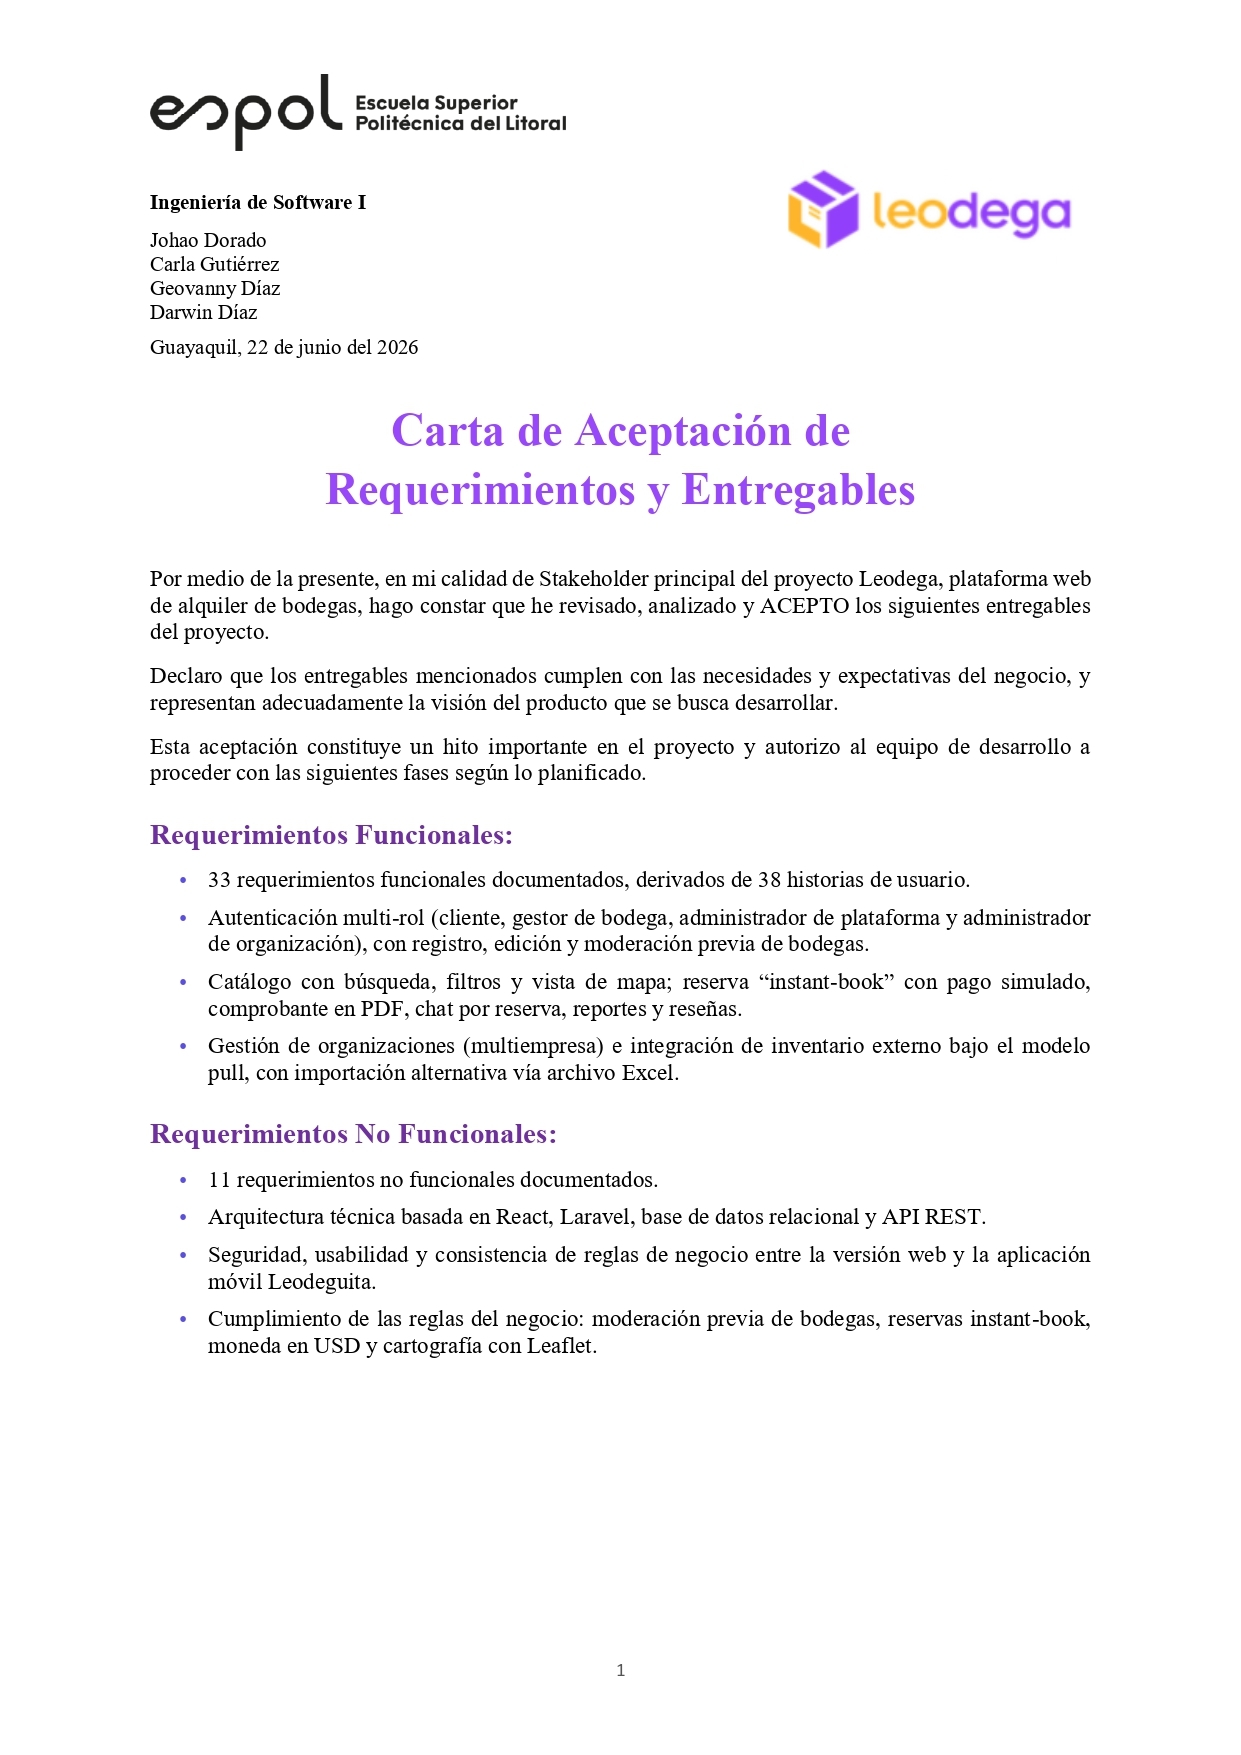
\includepdf[pages=-]{imagenes/acta_conformidad_ers.pdf}
}{%
  \begin{center}
  \fbox{\begin{minipage}[c][0.5\textheight][c]{0.9\textwidth}
    \centering\itshape\color{gray}
    Insertar aquí el acta de conformidad firmada correspondiente al ERS mejorado y al prototipo de alta fidelidad.\\
    (Archivo esperado: \texttt{imagenes/acta_conformidad_ers.pdf})
  \end{minipage}}
  \end{center}
}
